\section{Method: DocPC}
\label{sec:method}

\subsection{Overview}

DocPC represents each document by a small set of representative pages composed into a single grid image and scores it with a VLM and late interaction (Figure~\ref{fig:main-pipeline}). Given a document with $N$ pages, we select $K$ pages (Section~\ref{sec:page-composition}), compose them into a grid (2$\times$2 by default), and encode the grid once. At retrieval time we encode the query and compute similarity via late interaction (e.g., MaxSim). Training uses document-level supervision from the DocViRe training split (Section~\ref{sec:dataset}) with the objectives below. Because each document is encoded once as a fixed-size grid rather than indexed page by page, DocPC reduces document-side indexing to one representation per document. Quantitative efficiency results are reported in Section~\ref{sec:efficiency-footprint}.

\begin{figure*}[t]
  \centering
  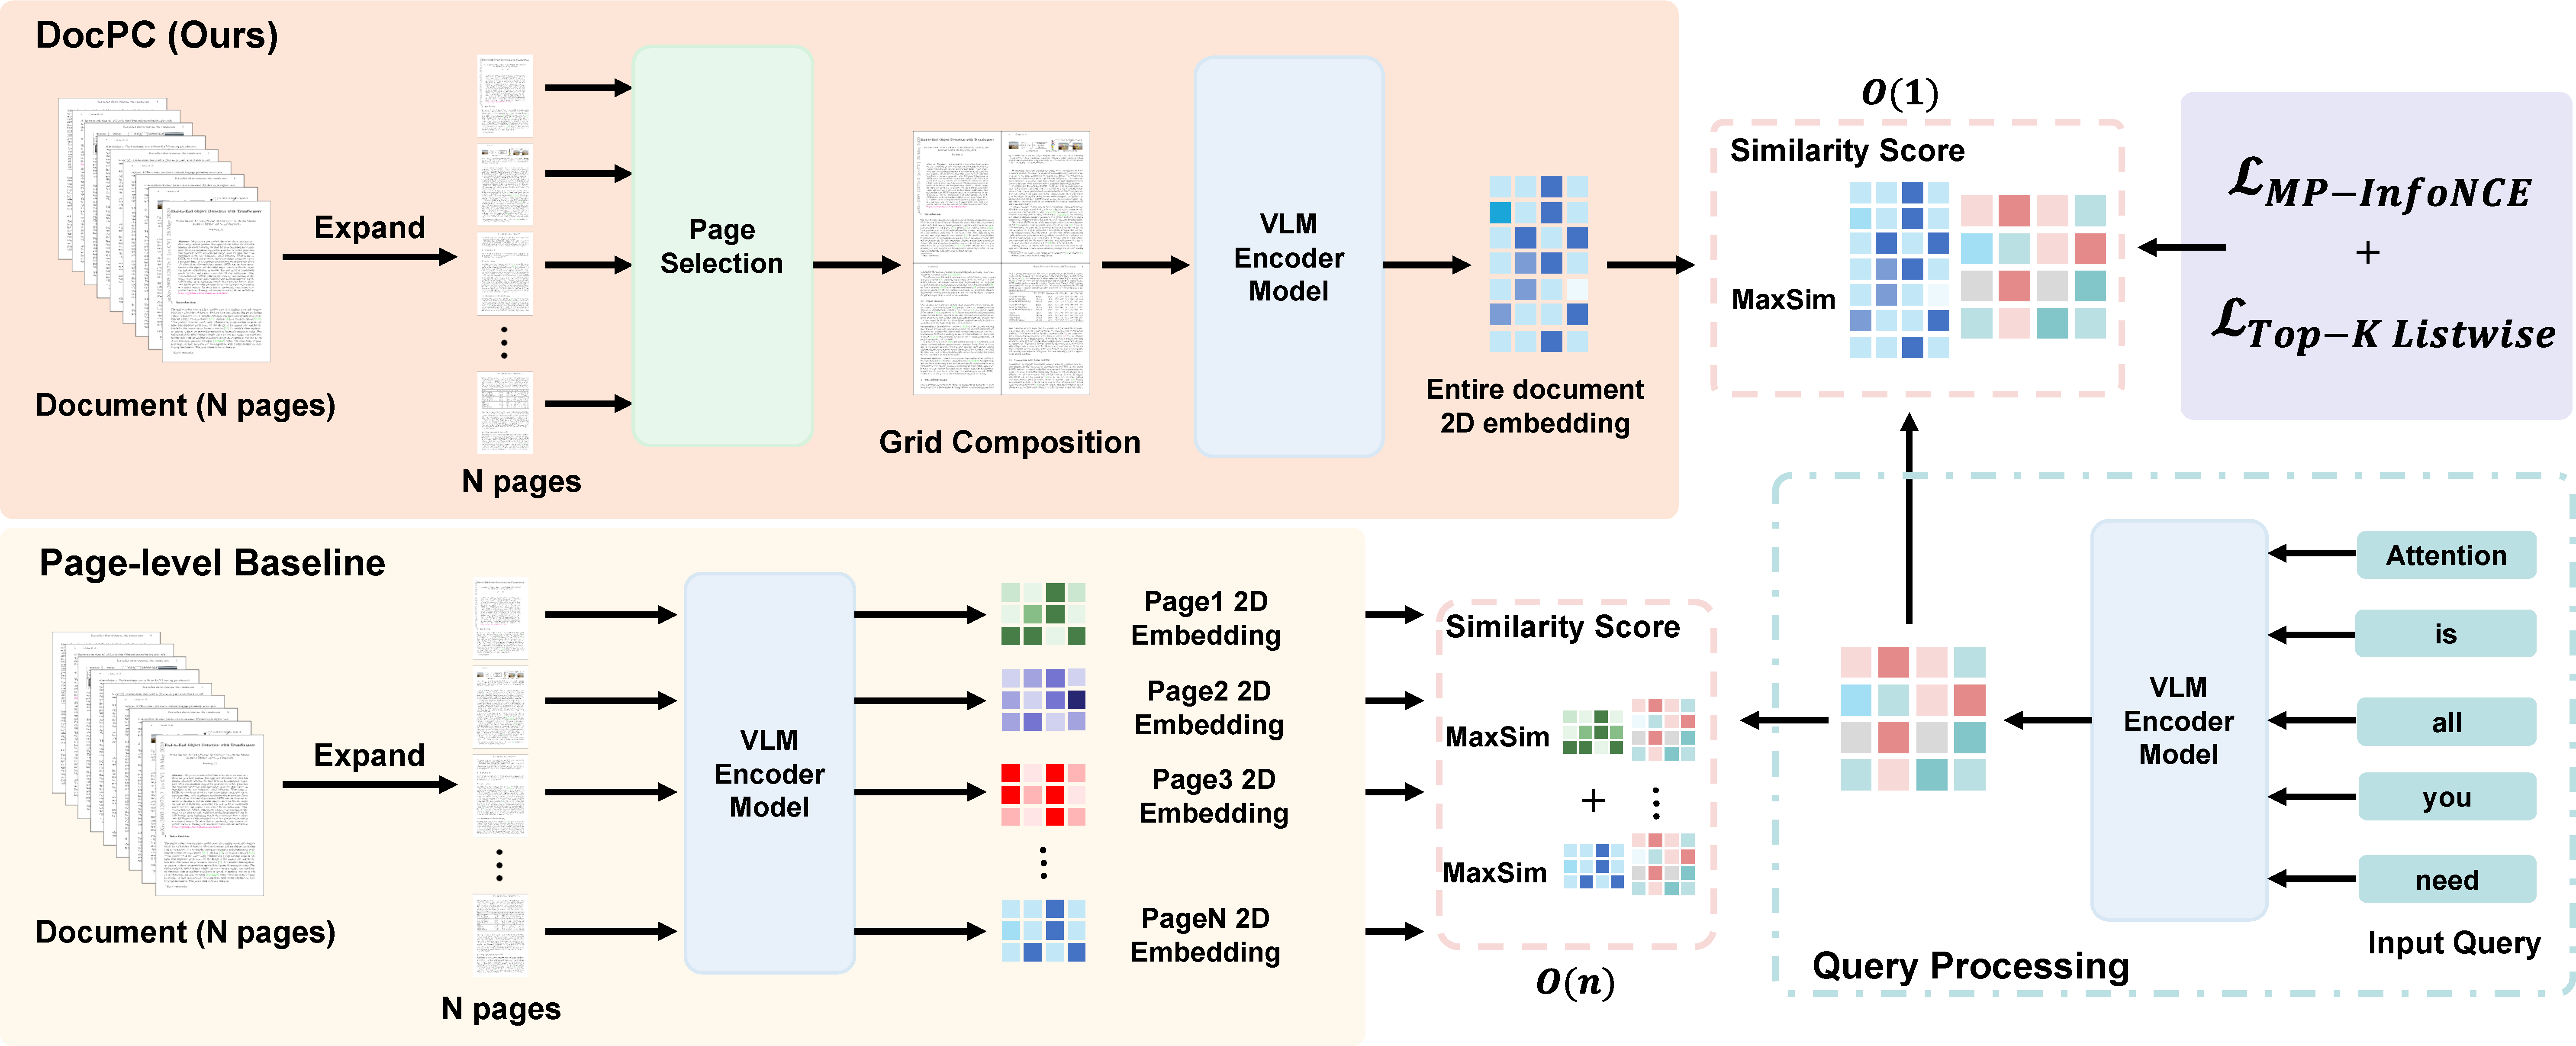
\includegraphics[width=\textwidth]{latex/figures/主流程.pdf}
  \caption{Overview of DocPC compared with the page-level baseline. \textbf{Top:} DocPC selects $K$ representative pages from a document, composes them into a single grid image (2$\times$2 by default), and encodes the grid once with the VLM to obtain an $\mathcal{O}(1)$ multi-vector document representation. \textbf{Bottom:} The page-level baseline encodes each page independently, producing $\mathcal{O}(N)$ embeddings per document, and aggregates per-page MaxSim scores at retrieval time. Both pipelines share the same query encoder with late interaction. Training combines Multi-Positive InfoNCE with a sparsely scheduled Top-$K$ listwise loss to handle multi-positive relevance.}
  \label{fig:main-pipeline}
\end{figure*}

\subsection{Representative Page Composition}
\label{sec:page-composition}

A core design choice is how to select $K$ pages to form the document's visual summary. Section~\ref{sec:task_formulation} shows that early pages tend to carry stronger signals. We consider both heuristic and embedding-based page selection strategies.

\textbf{First-$K$.} We take the first $K$ pages, which often contain highly informative front matter such as titles, opening sections, and tables of contents.

\textbf{Boundary.} We take the first $K/2$ and the last $K/2$ pages, targeting early and late document regions that often contain globally informative cues such as introductions, summaries, and conclusions.

\textbf{Uniform-$K$.} We sample $K$ pages at uniformly spaced indices (e.g., pages $1, \lfloor N/K \rfloor{+}1, \ldots, N$) to spread coverage across the document and avoid over-representing a single segment.

\textbf{Random-$K$.} We randomly sample $K$ pages, providing a baseline with no structural prior.

\textbf{Base-Clip.} We also consider an embedding-based dynamic page selection strategy. We first compute CLIP embeddings for all candidate pages \citep{pmlr-v139-radford21a}, cluster them, and select four representative pages from clusters to compose the final grid. Unlike fixed heuristics, this strategy selects pages according to document-specific visual-semantic structure and is used in ablation (Table~\ref{tab:page-budget}) to compare against heuristic First-4 selection.

By default we set $K=4$ and arrange the selected pages in a $2{\times}2$ grid. We use the following layouts in our experiments: $K{=}1$ gives a single-page ($1{\times}1$) representation. $K{=}4$ gives a four-page $2{\times}2$ grid. $K{=}16$ gives a 16-page larger grid. In all cases, pages are resized to a common resolution by the VLM preprocessing pipeline and arranged into a single grid image before being fed to the encoder. Thus, each document is represented by a fixed-size grid regardless of its total page count. By default we use the First-4 grid as the primary configuration. We also consider Boundary and Base-Clip as alternative page selection strategies.

\subsection{Training Objectives}
\label{sec:training-objectives}

Document-level retrieval introduces two training challenges: multiple positive documents per query (multi-positive) and the need to optimize the ranking of top-$K$ results. We address them with two losses.

\textbf{Multi-Positive InfoNCE.} Contrastive learning for visual and multimodal representations is well established \citep{pmlr-v119-chen20j,He_2020_CVPR,oord2018infonce}. Standard contrastive losses (e.g., InfoNCE) assume one positive pair per query. In document-level benchmarks like DocViRe, a query can have multiple relevant documents. Treating other positives in the batch as negatives hurts training. To relax the ``one query, one positive'' assumption, we use a multi-positive InfoNCE objective, similar in spirit to prior MP-InfoNCE formulations \citep{rivas2024conked}, that aggregates over the positive set $\mathcal{P}$ and keeps negatives in $\mathcal{N}$:
\begin{equation}
\mathcal{L}_{\mathrm{MP}\mbox{-}\mathrm{InfoNCE}} = -\log \frac{S_{\mathcal{P}}}{S_{\mathcal{P}} + S_{\mathcal{N}}},
\label{eq:mp-infonce}
\end{equation}
where $S_{\mathcal{P}} = \sum_{i \in \mathcal{P}} \exp(\mathrm{sim}(q, d_i^+) / \tau)$ and $S_{\mathcal{N}} = \sum_{j \in \mathcal{N}} \exp(\mathrm{sim}(q, d_j^-) / \tau)$. Here $\mathrm{sim}(q, d)$ is the late-interaction similarity, $\tau$ is the temperature, $d_i^+$ are positives and $d_j^-$ are negatives. This encourages the query to be close to all positives while pushed away from negatives.

\textbf{Top-$K$ listwise loss.} To directly optimize the quality of the top-$K$ ranking, we use a listwise loss based on ApproxNDCG \citep{qin2010general}, which is differentiable and focuses on the top positions:
\begin{equation}
\mathcal{L}_{\mathrm{top}\mbox{-}k} = 1 - \mathrm{ApproxNDCG}(\mathbf{y}, \mathbf{r}, K),
\label{eq:topk-loss}
\end{equation}
where $\mathbf{y}$ and $\mathbf{r}$ denote predicted scores and relevance labels.
Minimizing $\mathcal{L}_{\mathrm{top}\mbox{-}k}$ improves the ordering of the top-$K$ list relative to the relevance labels. Prior work in image retrieval has also optimized ranking metrics with listwise losses \citep{Revaud_2019_ICCV}.

\textbf{Combined objective.} We train with a weighted combination:
\begin{equation}
\mathcal{L} = \mathcal{L}_{\mathrm{MP}\mbox{-}\mathrm{InfoNCE}} + \lambda \,\mathcal{L}_{\mathrm{top}\mbox{-}k},
\label{eq:combined-loss}
\end{equation}
where $\lambda$ balances the contrastive and listwise terms. In practice, the multi-positive loss is applied at every step, while the listwise term is introduced intermittently during training. The multi-positive loss reduces false negatives among relevant documents, and the listwise loss refines the ranking of the top results.

\subsection{Training and Inference}

\textbf{Training.} We start from a pretrained page-level retrieval model ColQwen, apply the representative page composition to each document in the training set, and fine-tune on DocViRe using the combined loss $\mathcal{L}$. In-batch negatives are used for the contrastive term. No extra negative sampling is required.

\textbf{Inference.} Offline indexing is done once per document: compose a grid from the selected pages (2$\times$2 by default), run a single VLM forward pass, and store the multi-vector representation. At query time, we encode the query once, compute late-interaction scores against all document representations, and return the top-ranked documents.

\begin{table*}[!t]
  \centering
  \footnotesize
  \setlength{\tabcolsep}{4pt}
  \caption{Main results on DocViRe (NDCG@5, \%) per domain and average. Text-only baselines use OCR text or LLM-generated document summaries. Page-level VLM baselines index individual pages and aggregate with MaxP. Document-level methods use a single 4-page grid per document. For model names with two tags, the first tag denotes the training setting and the second denotes the test-time page or grid strategy. DocPC-ColQwen (First-4) uses the First-4 grid as the best configuration (see Section~\ref{sec:ablation}). Overall best in bold.}
  \label{tab:main-results}
  \begin{tabular}{@{}lrrrrrrrr@{}}
    \toprule
    Model & Bio. & Edu. & Fin. & Gov. & Ind. & Leg. & Res. & Avg \\
    \midrule
    \multicolumn{9}{@{}l}{\itshape Text-only} \\
    \midrule
    \textsc{BGE-M3} & 41.30 & 39.77 & 20.59 & 23.13 & 31.61 & 29.09 & 47.95 & 33.35 \\
    \textsc{BM25}   & 35.36 & 37.48 & 24.08 & 19.94 & 33.35 & 29.96 & 46.97 & 32.45 \\
    BGE-M3 (LLM sum.) & 36.32 & 41.07 & 15.94 & 25.92 & 34.61 & 34.19 & 50.18 & 34.03 \\
    BM25 (LLM sum.)   & 31.96 & 40.17 & 17.96 & 24.06 & 35.76 & 34.18 & 44.79 & 32.70 \\
    \midrule
    \multicolumn{9}{@{}l}{\itshape Page-level VLM baselines} \\
    \midrule
    ColQwen-page (zero-shot, All pages)& \underline{50.98} & 33.92 & 22.83 & 27.04 & 10.02 & 37.98 & 56.40 & 34.17 \\
    ColQwen-page (zero-shot, Boundary) & \textbf{52.89} & 34.20 & 22.89 & 26.54 & 8.52 & 40.58 & 56.48 & 34.59 \\
    ColQwen-page (DocViRe-sft, All pages) & 46.01 & 37.90 & 30.36 & 30.89 & 20.53 & 44.78 & \underline{56.65} & 38.16 \\
    ColQwen-page (DocViRe-sft, Boundary) & 47.09 & 38.78 & \underline{32.18} & \underline{31.93} & 20.39 & \underline{46.51} & \textbf{57.42} & 38.91 \\
    \midrule
    \multicolumn{9}{@{}l}{\itshape Document-level VLM (4-page grids)} \\
    \midrule
    Jina-CLIP (zero-shot, First-4) & 20.35 & 23.86 & 10.92 & 10.10 & 25.18 & 13.20 & 31.36 & 19.28 \\
    Nomic-Embed (zero-shot, First-4) & 4.90 & 6.96 & 8.98 & 1.74 & 16.06 & 0.73 & 10.40 & 7.11 \\
    ColQwen (DocViRe-sft, First-4) & 42.24 & \textbf{46.86} & 30.22 & 31.93 & \underline{41.11} & 42.40 & 50.47 & \underline{40.75} \\
    \midrule
    \multicolumn{9}{@{}l}{\itshape Ours} \\
    \midrule
    \textbf{DocPC-ColQwen (First-4)} & 49.02 & \underline{46.44} & \textbf{33.46} & \textbf{33.25} & \textbf{47.44} & \textbf{46.64} & 52.41 & \textbf{44.09} \\
    \bottomrule
  \end{tabular}
\end{table*}